% --------------------------------------
% Document Class
% --------------------------------------
\documentclass[a4paper,11pt]{article}
% --------------------------------------



% --------------------------------------
% Use Package
% --------------------------------------


\usepackage[francais]{babel}
\usepackage{ucs}
\usepackage[utf8]{inputenc}
\usepackage[T1]{fontenc}

\usepackage{makeidx}
\usepackage{color}
\usepackage{graphicx}
\usepackage{float}
\usepackage[hidelinks]{hyperref} 
\usepackage{geometry}
%\usepackage{lastpage}
%\usepackage{marginnote}
\usepackage{fancyhdr}
%\usepackage{titlesec}
%\usepackage{framed}
\usepackage{amsmath}
\usepackage{empheq}
\usepackage{array}
\usepackage{multicol}
\usepackage{csquotes}
%\usepackage{adjustbox}

% insert code
\usepackage{listings}

% define our color
\usepackage{xcolor}

% code color
\definecolor{ligthyellow}{RGB}{250,247,220}
\definecolor{darkblue}{RGB}{5,10,85}
\definecolor{ligthblue}{RGB}{1,147,128}
\definecolor{darkgreen}{RGB}{8,120,51}
\definecolor{darkred}{RGB}{160,0,0}

% other color
\definecolor{ivi}{RGB}{141,107,185}

\def\verticaltext#1{\rotatebox[origin=c]{90}{\x{#1}}}


\lstset{
    language=python,
    captionpos=b,
    extendedchars=true,
    frame=lines,
    numbers=left,
    numberstyle=\tiny,
    numbersep=5pt,
    keepspaces=true,
    breaklines=true,
    showspaces=false,
    showstringspaces=false,
    breakatwhitespace=false,
    stepnumber=1,
    showtabs=false,
    tabsize=3,
    basicstyle=\small\ttfamily,
    backgroundcolor=\color{ligthyellow},
    keywordstyle=\color{ligthblue},
    morekeywords={include, printf, uchar},
    identifierstyle=\color{darkblue},
    commentstyle=\color{darkgreen},
    stringstyle=\color{darkred},
}


% --------------------------------------



% --------------------------------------
% Page setting
% --------------------------------------
%\pagestyle{empty}
\setlength{\headheight}{15pt}

\setcounter{secnumdepth}{3}
\setcounter{tocdepth}{2}

\makeatletter
\@addtoreset{chapter}{part}
\makeatother 

\hypersetup{       % parametrage des hyperliens
  colorlinks=true,  % colorise les liens
  breaklinks=true,  % permet les retours à la ligne pour les liens 
                    % trop longs
  urlcolor= blue,   % couleur des hyperliens
  linkcolor= black, % couleur des liens internes aux documents 
                    % (index, figures, tableaux, equations,...)
  citecolor= green  % couleur des liens vers les references 
                    % bibliographiques
}

% --------------------------------------

% --------------------------------------
% Information
% --------------------------------------
\title{
  \noindent\hrulefill \\
  \vspace{10mm}
  \textbf{Compte-rendu VisA} \\
  \vspace{5mm}
  TP: Modification de la luminance et la saturation d'une image couleur.
}

\author{Gaëtan DEFLANDRE}
% --------------------------------------

\definecolor{myColor}{rgb}{0.5, 0.1, 0.75}

% --------------------------------------
% Begin content
% --------------------------------------
\begin{document}

\maketitle
\noindent\hrulefill \\


\section*{Introduction}


\newpage

Dans ce TP, nous travaillons avec les images du test d'Ishihara utilisé 
pour déceler le daltonisme.

\begin{figure}[H]
  \begin{center}
    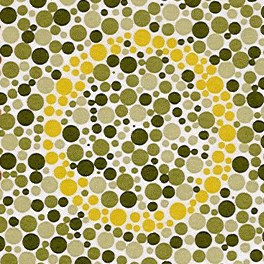
\includegraphics[width=120px]{images/it1_72pp.png}
    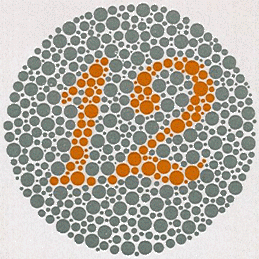
\includegraphics[width=120px]{images/it2_72pp.png}
    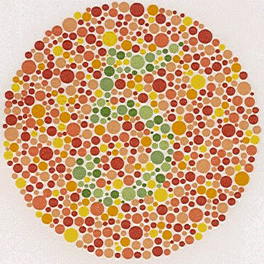
\includegraphics[width=120px]{images/it3_72pp.png}
    \caption{Images originales utiles à ce TP}
  \end{center}
\end{figure}

\section{Manipulation de la luminance}

Dans cet exercice, nous utilisons les images d'origine assombries:

\begin{figure}[H]
  \begin{center}
    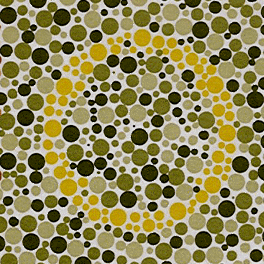
\includegraphics[width=120px]{images/it1_72pp_sombre.png}
    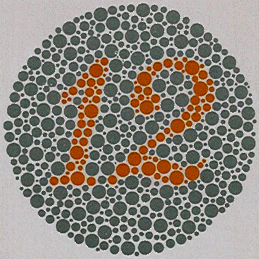
\includegraphics[width=120px]{images/it2_72pp_sombre.png}
    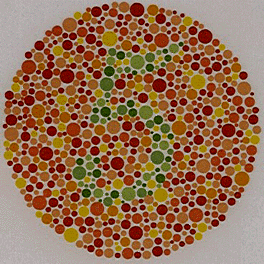
\includegraphics[width=120px]{images/it3_72pp_sombre.png}
    \caption{Images sombres}
  \end{center}
\end{figure}

Pour retrouver, de manière précise, les différences entre l'image 
d'origine et l'image assombrie, il faut choisir le bon espace de
représentation de l'image. Dans notre cas, seule la luminosité 
semble avoir été modifié, ainsi pour trouver aisément cette 
différence, nous choisissons un espace qui contient l'information de 
luminance.\\

Les espaces tels que \textit{Lab} et \textit{Luv} contiennent cette 
information. La valeur \textit{V} de l'espace \textit{HSV} ou le 
\textit{Y} de l'espace \textit{YUV} peuvent être utilisé. Nous 
nous servons de l'espace \textit{Lab} lors de cet exercice.\\

Nous pourrions regarder l'information de chrominance également, 
afin de voir si celle-ci a été modifié.\\

\begin{figure}[H]
  \begin{center}  
    \shortstack{
      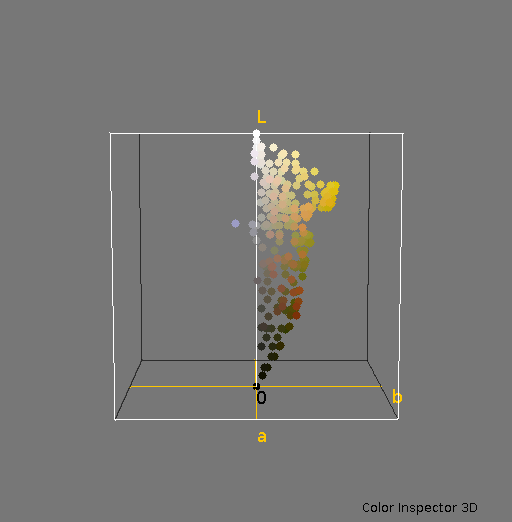
\includegraphics[width=150px]{images/it1.png} \\ 
      \texttt{\small it1\_72pp.png}
    }
    \shortstack{
      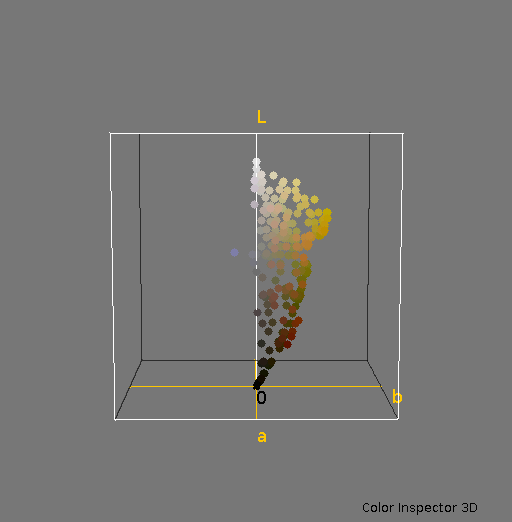
\includegraphics[width=150px]{images/it1_sombre.png}\\
      \texttt{\small it1\_72pp\_sombre.png}
    }
    \caption{Diagrammes de it1 original et assombri dans l'espace Lab.}
  \end{center}
\end{figure}

Dans l'espace \textit{Lab}, on voit nettement la différence sur l'axe 
de la luminance. La luminance de l'image sombre ne va pas dans les 
tons très clairs, alors que la luminance de l'image d'origine est 
réparti sur tout l'axe \textit{L}.\\

Ainsi, nous pouvons retrouver une valeur $\varphi$ à ajouter à chaque 
canal de \textit{RGB} pour que les images sombres approximent les images
originales.



\begin{table}[H]
  \begin{center}
  
    \begin{tabular}{|l||c|c|c|}
    
      \hline
    
      \bf Images originales &
      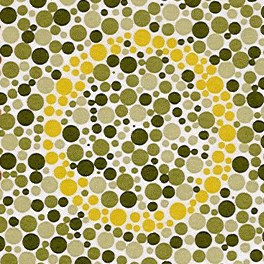
\includegraphics[width=80px]{images/it1_72pp.png} & 
      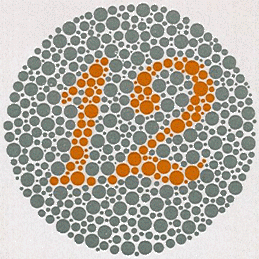
\includegraphics[width=80px]{images/it2_72pp.png} & 
      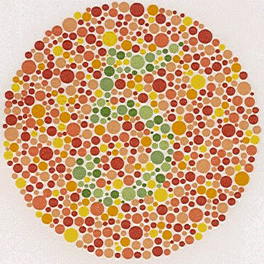
\includegraphics[width=80px]{images/it3_72pp.png} \\
      
      \hline
       
      \bf Images sombres &
      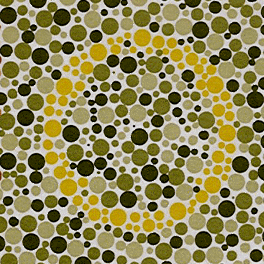
\includegraphics[width=80px]{images/it1_72pp_sombre.png} &
      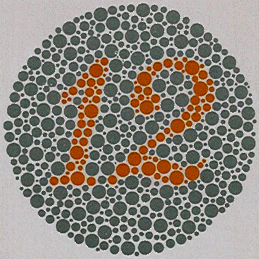
\includegraphics[width=80px]{images/it2_72pp_sombre.png} &
      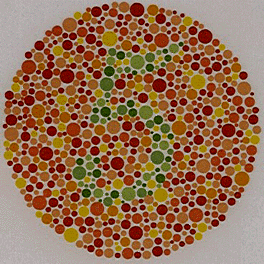
\includegraphics[width=80px]{images/it3_72pp_sombre.png}\\
      
      \hline
      
      \bf Valeur de $\varphi$ &
      30 &
      40 &
      60\\
      
      \hline
    \end{tabular}
    
    \caption{Tableau des valeurs de $\varphi$}
    \label{tab:}
    
  \end{center}
\end{table}

Cependant lorsqu'on calcule la différence entre l'image originale et 
l'image résultante après ajout de la valeur $\varphi$. On remarque que 
les images ne sont pas identiques.

\begin{figure}[H]
  \begin{center}  
    \shortstack{
      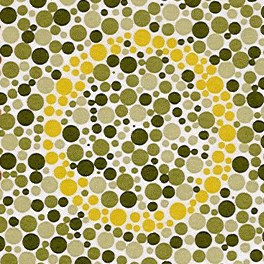
\includegraphics[width=120px]{images/it1_72pp.png} \\ 
      \texttt{\small it1\_72pp.png}
    }
    \shortstack{
      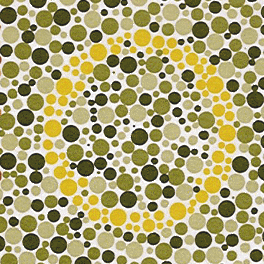
\includegraphics[width=120px]{images/luminance_it1.png}\\
      {\small \texttt{it1\_72pp\_sombre.png} + $\varphi$ }
    }\\
    \shortstack{
      
\includegraphics[width=120px]{images/diff_it1.png}\\
      {\small Différence}
    }
    \shortstack{
      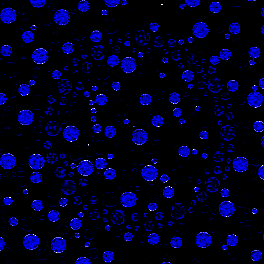
\includegraphics[width=120px]{images/diff_it1_norm.png}\\
      {\small Différence normalisée}
    }
    \caption{La référence non identique}
  \end{center}
\end{figure}

Cette différence est normale comme nous ajoutons la même valeur pour 
chaque canal dans l'espace \textit{RGB}. Or seule la luminance semble
avoir été modifié. Pour régler ce problème, il faut ajouter la valeur 
$\varphi$ à la luminance dans un espace qui la contient. 

\section{Rétablissement de la saturation}

\section{Exercice 3}

\section{Exercice 4}

\section*{Conclusion}


\end{document}
